\documentclass{beamer}

\usepackage{graphicx}
%\usepackage{epstopdf}
\usepackage{color}
\usepackage{textcomp}

% Import the UNCMath theme.
% UNC is the default color theme.
\usetheme{UNCMath}

% Uncomment to use a different color scheme.
%\definecolor{darkpurple}{rgb}{0.2,0,0.2}
%\setbeamercolor*{structure}{fg=black,bg=darkpurple}

\logo{

\includegraphics[height=3em]{oldwell_cmyk}
}

% A macro for making the title frame.
% Removes the bottom bar and logo temporarily.
% If you don't want these in other frames, 
% you could try mimicking this.
\newcommand{\titleframe}{
{
\setbeamertemplate{headline}{}
\setbeamertemplate{footline}{}
\begin{frame}
\titlepage
\end{frame}
}
}

%\renewcommand*{\bibfont}{\scriptsize}


%%%%%%%%%%%%%%%%%%%%%%%%%%%%%%%%%%%%%%%%%%
%
% Information for the title frame.
%
\title{Identification of Schizophrenia Using Hippocampal Curvedness and Shape Index with Deep Learning}
\subtitle{COMP 766 Final Project}
\author[Siyang Jing]{
Siyang Jing
}
\institute{Department of Computer Science, UNC Chapel Hill}
\date{May 13th, 2019}

\begin{document}
\titleframe

\begin{frame}
\frametitle{Schizophrenia and Hippocampus}

\begin{itemize}
\item The hippocampus is one of the most extensively studied regions of the brain, with well-described anatomy and basic physiology; it's also closely related to human memory. 
\item In schizophrenia, alterations in hippocampal anatomy are consistently reported.
\item In particular, hippocampal volume reduction is now one of the most consistent structural abnormalities found in schizophrenia as it is present at the onset of the illness.
\end{itemize}
\end{frame}

\begin{frame}
\frametitle{SPHARM-PDM}
\begin{columns}
\begin{column}{0.5\textwidth}
A boundary PDM is a tuple of boundary points on an object, with points corresponding across the training cases.Hierarchical. SPHARM stands for spherical harmonics.
\begin{itemize}
    \item Surface \& Parameterization
    \item Fit coefficients of parameterized basis functions to surface
    \item Reconstruct object
\end{itemize}
\end{column}
\begin{column}{0.5\textwidth}
\begin{center}
    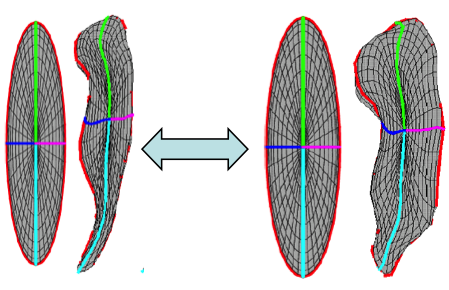
\includegraphics[width=0.5\linewidth]{SPHARM1.png}
\end{center}
\begin{center}
    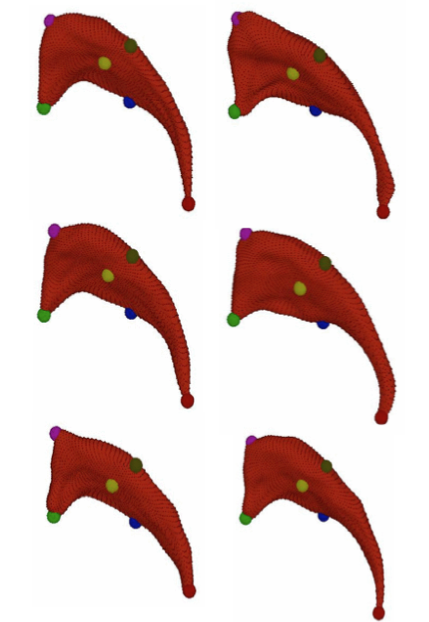
\includegraphics[width=0.5\linewidth]{SPHARM2.png}
\end{center}
\end{column}
\end{columns}
\end{frame}

\begin{frame}
\frametitle{Koenderink Curvedness and Shape Index}
\begin{columns}
\begin{column}{0.5\textwidth}
\begin{itemize}
    \item $s = \frac{2}{\pi}\arctan\frac{\kappa_2 + \kappa_1}{\kappa_2 - \kappa_1}$
    \item $s=\pm 1$: umbilics
    \item $s=\pm 0.5$: parabolic points
    \item $s\in(-1,-0.5)$: concave regions
    \item $s\in(-0.5,0.5)$: hyperbolic regions
    \item $s\in(0.5,1)$: convex regions
    \item $c = \sqrt{\frac{\kappa_1^2 + \kappa_2^2}{2}}$
    \item $c$ describes how ``curved"" the surface is
\end{itemize}
\end{column}
\begin{column}{0.5\textwidth} 
    \begin{center}
    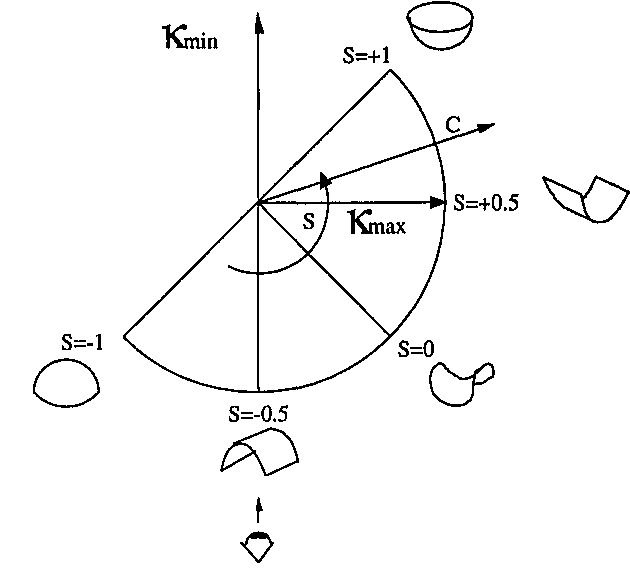
\includegraphics[width=0.8\linewidth]{CandS.png}
    \end{center}
\end{column}
\end{columns}

\end{frame}

\begin{frame}
\frametitle{Data}
\begin{itemize}
    \item In this project, I study the problem of classifying hippocampi as schizophrenic or healthy.
    \item Original data include 238 schizophrenic subjects and 56 healthy subjects.
    \item Data were provided to me as $256\times 3$ spharm coefficients.
    \item The boundary PDMs of $C$ and $S$ and $K$ and $H$ are calculated using SPHARM-PDM Toolbox with 1002 points.
    \item In processing, SpharmTool reported umbilics in some cases and those cases are discarded.
    \item SlicerSalt is used to calculate the volumes and flip the left hippocampi to the right for convolution.
\end{itemize}
\end{frame}

\begin{frame}
\frametitle{Data}
\begin{columns}
\begin{column}{0.5\textwidth}
    \begin{center}
    Schizophrenic Case: $2946$ mm\textsuperscript{3}\\
    C: 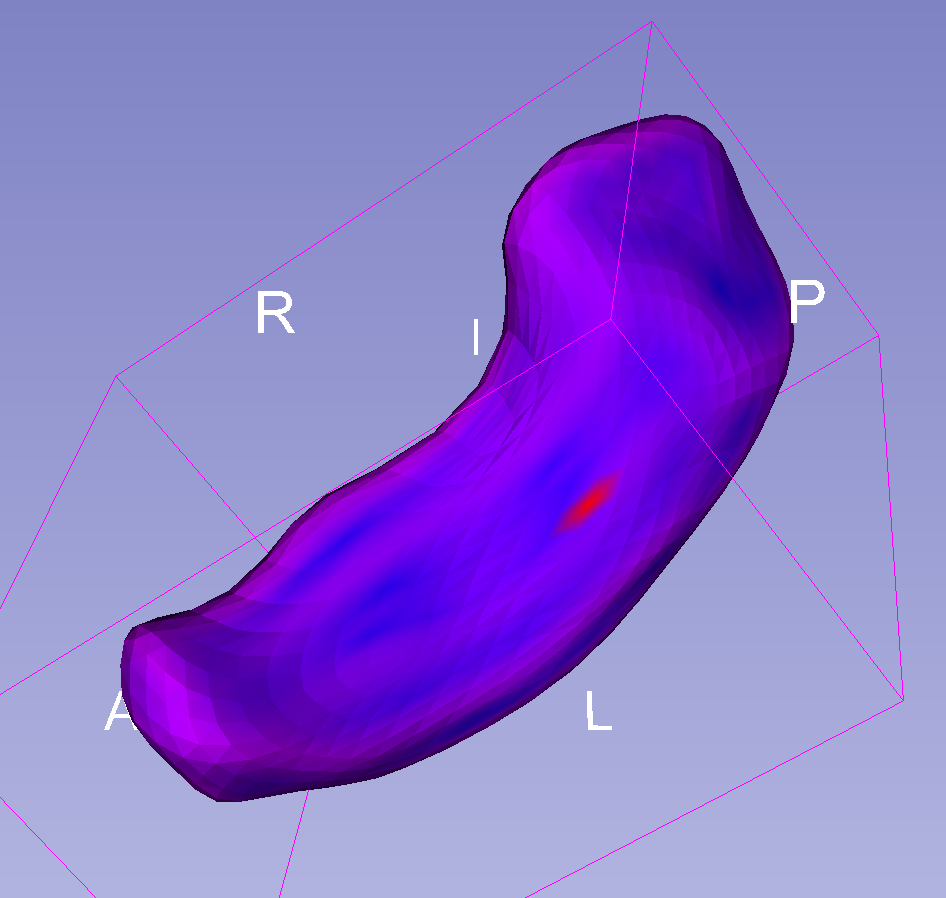
\includegraphics[width=0.5\linewidth]{YC.png}\\
    S: 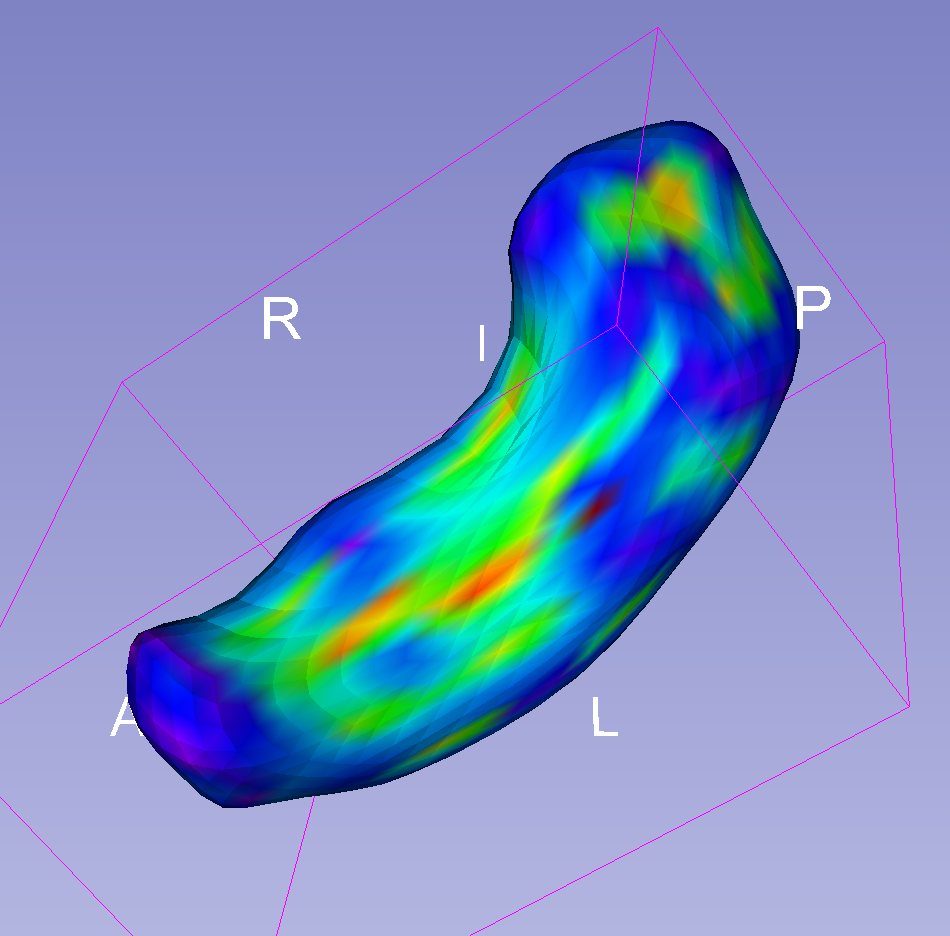
\includegraphics[width=0.5\linewidth]{YS.png}
    \end{center}
\end{column}
\begin{column}{0.5\textwidth} 
    \begin{center}
    Healthy Case: $3384$ mm\textsuperscript{3}\\
    C: 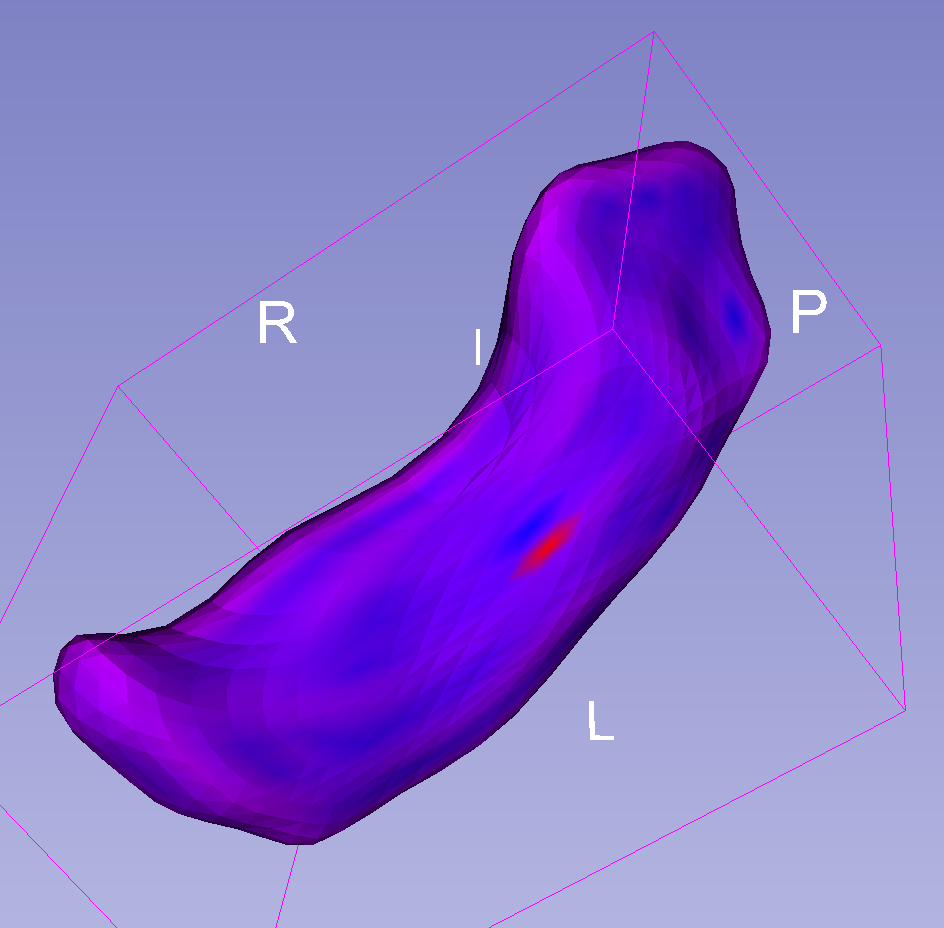
\includegraphics[width=0.5\linewidth]{NC.png}\\
    S: 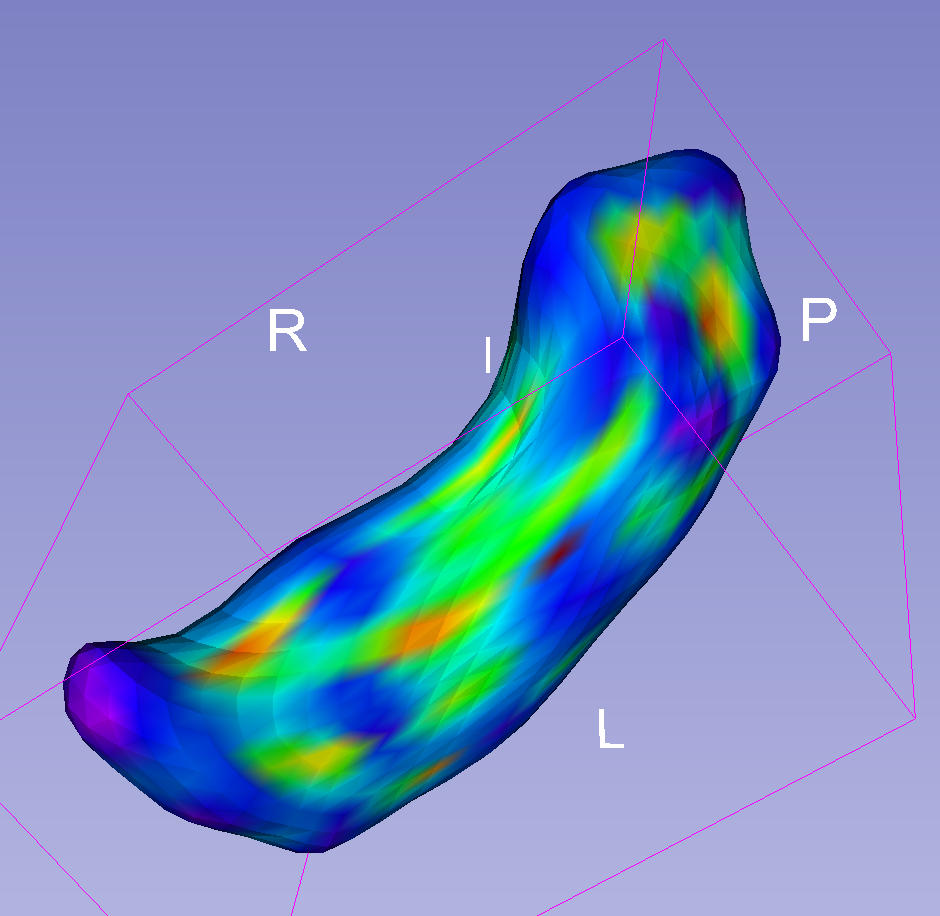
\includegraphics[width=0.5\linewidth]{NS.png}
    \end{center}
\end{column}
\end{columns}

\end{frame}

\begin{frame}
\frametitle{Previous Approaches}
\begin{itemize}
    \item Skeletal representations (s-reps)
    \begin{itemize}
        \item Junpyo Hong proposed a method based on skeletal representations (s-reps).
        \item distance weighted discrimination (DWD) with
        \item Euclideanization with Principal Nested Spheres (PNS)
    \end{itemize}
    \item Boundary point distribution model (PDM)
    \begin{itemize}
        \item Principal Component Analysis (PCA)
        \item Support Vector Machine (SVM)
        \item Proposed: neural networks
    \end{itemize}
\end{itemize}
\end{frame}

\begin{frame}
\frametitle{Method: Fully Connected Network}
\scriptsize{
\begin{itemize}
    \item Fully connected network is the simplest structure where no weights are shared between features. It is also easy to implement with a few lines of code. \\
    \item I started with using C and S for left and right hippocampi, with $8004$ features in total. I also experimented with using both $C$ and $S$, and $K$ and $H$ for left and right hippocampi, with $16008$ features in total. \\
    \item Although $C+S$ and $K+H$ are mutually derivable, more features might provide more information to the model and make the classification more accurate.
\end{itemize}
}
\begin{center}
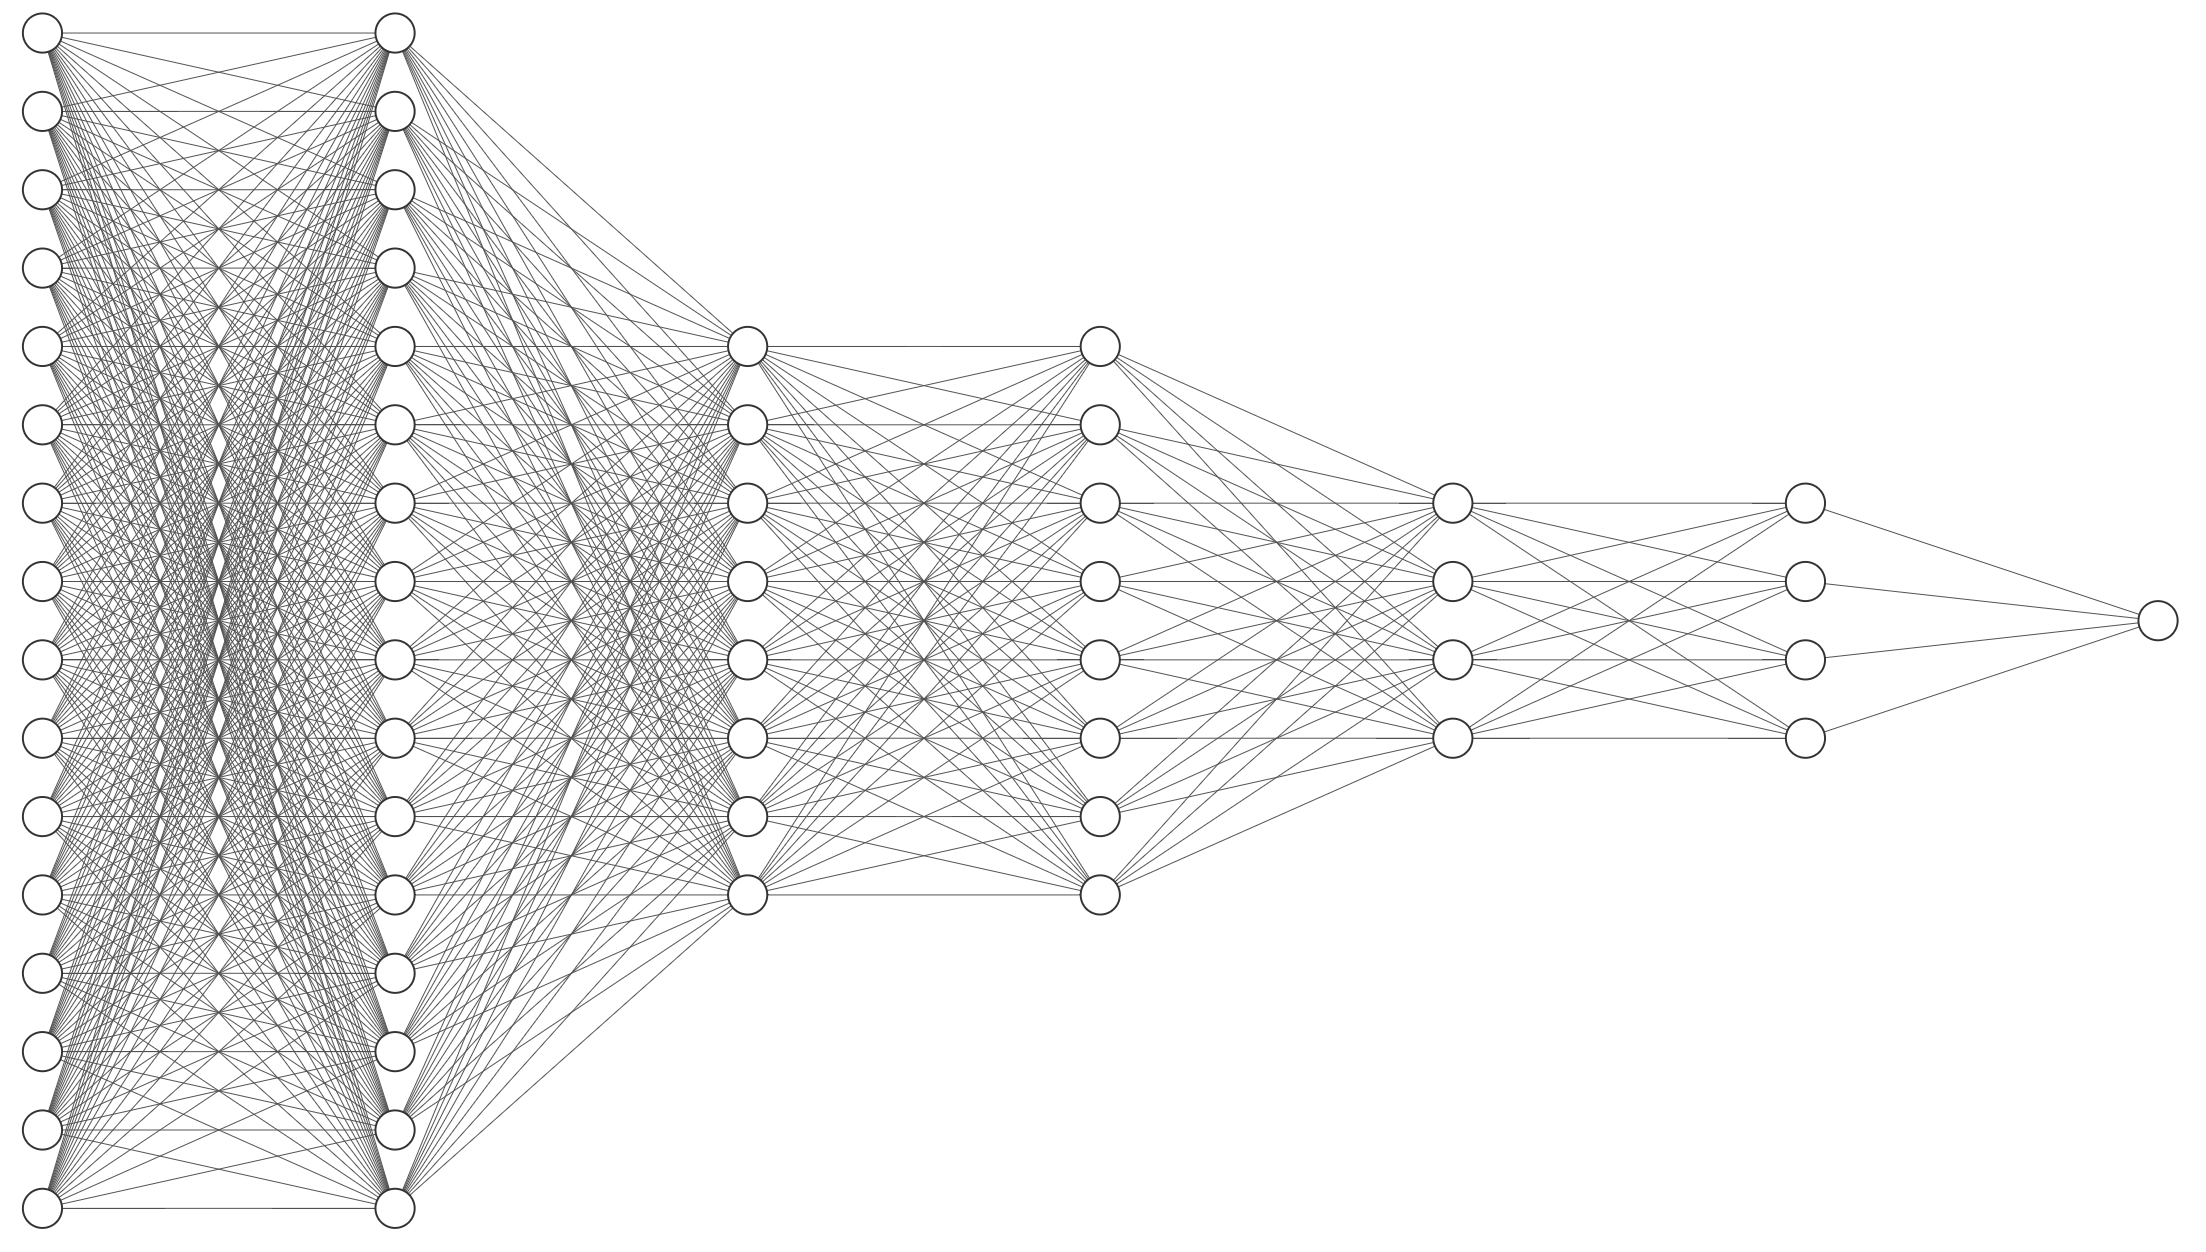
\includegraphics[width=0.7\linewidth]{FCN.png}
\end{center}
\end{frame}

\begin{frame}
\frametitle{Method: 1D CNN}
\scriptsize{
\begin{itemize}
    \item Consider $C$ and $S$ of left and right hippocampi as $4$ channels and regard the SPHARM-PDM of each feature map as a 1-dimensional array. 1D CNN seems a reasonable choice for such data structure.
    \item I was trying to use spherical CNNs but failed to build a robust implementation due to time constraint.
    \item After some experiment, the filter size was selected as $20$.
    \item Each convolution layer is followed by a pooling layer with $10$ pairs in total. Two fully connected layers are added to the end. The output layer uses softmax to give the prediction.
    \item Below is a picture for illustration. It does not represent the proposed structure.
\end{itemize}
}
\centering
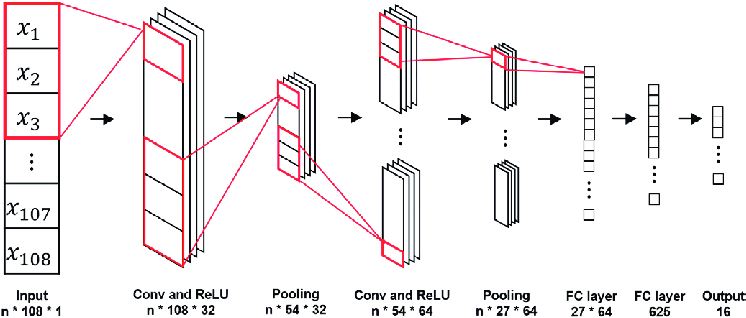
\includegraphics[width=0.8\linewidth]{1Dconv.png}
\end{frame}

\begin{frame}
\frametitle{Training}
\begin{itemize}
    \item The negative cases are duplicated so that the effective number of positive and negative cases in the training set and the test set are equal.
    \item The model is implemented in keras with default training parameters for $200$ epochs.
\end{itemize}
\end{frame}

\begin{frame}
\frametitle{Results}
The probabilities are predicted and the ROC and AUC are generated with \texttt{sklearn.metrics}.
\begin{center}
\begin{tabular}{|c|c|c|}\hline
Methods & AUC & Confidence intervals \\ \hline
(Hong et.al. 2016): s-reps & 0.6457 & [0.6363, 0.6551] \\ \hline
1D convolution: C and S + K and H & 0.5633 & [0.5532, 0.5701] \\ \hline
1D convolution: C and S & 0.5620 & [0.5547, 0.5670] \\ \hline
C and S + K and H + Volume & 0.5711 & [0.5524, 0.5968] \\ \hline
C and S + K and H & 0.5689 & [0.5571, 0.5734] \\ \hline
C and S + Volume & 0.5671 & [0.5425, 0.5839] \\ \hline
C and S& 0.5645 & [0.5605, 0.5762] \\ \hline
Volume& 0.5202 & [0.5042, 0.5451] \\ \hline
Random guessing & 0.5000 & [0.4964, 0.5037] \\ \hline
\end{tabular}
\end{center}
\end{frame}

\begin{frame}
\frametitle{Thanks!}
\begin{itemize}
    \item Thank Prof. Martin Styner for providing the data and teaching me how to use the tools and softwares.
    \item I also stole the pictures of SPHARM-PDM from Prof. Martin Styner's old slides.
    \item Beamer template from Manuchehr Aminian (https://github.com/maminian/uncmathbeamer).
\end{itemize}
\vspace{1em}

\begin{figure}
\centering

\includegraphics[width=0.5\linewidth]{oldwell_cmyk}
\end{figure}
\end{frame}

\end{document}
